\chapter{Topic Modeling}

In Chapter \ref{wordemb}, we presented some techniques to encode words as vectors.
Starting from a bag-of-words model in which we assume that the order of the words
inside a text does not matter, it is possible to follow a similar approach also for documents.
Topic models play an important role in describing, organizing and comparing unstructured collections of documents.

The first step is to generate a matrix of term counts $X$ for the entire corpus:
each row is a document represented in the BOW format and each column represents the count of occurrence
of a particular term in the documents.

The goal of the second step is to produce two matrices:
\begin{itemize}
    \item \textbf{term-topic matrix}: each row represents how related each term is to all topics
    \item \textbf{document-topic matrix}: each row represents how related each document is to all topics
\end{itemize}

For instance, a document about bears is likely to have high intensity on some topics which in turn have high
intensity on words related to animals; see Figure \ref{fig:topicmat} for an example.

\section{Latent Semantic Analysis (LSA)}
Given the number of topics $V$ as an hyperparameter,
Truncated SVD is applied to the matrix obtained in the first step
(see Figure \ref{fig:svd} for a graphical representation):
\[X_{N \times K} = U_{N \times V} \Sigma_{V \times V} D_{K \times V}^T\]

The matrix $U$ is then used as the document-topic matrix,
while $D$ represents the term-topic matrix.

Using $U$ instead of $X$ for comparing documents when $V \ll K$ leads to a smaller memory footprint.
Furthermore, the terms are no longer orthogonal: thanks to this it is possible to compute the similarity between
a term and a document even if the document does not contain the term itself.
The key point to observe is that both terms and documents are described as topics: if a term is frequent in some topics and
a document is frequent in the same topics, they will have a similar representation in the new space.

An overview of this technique can be found at \cite{doi:10.1002/aris.1440380105}.

\begin{figure}[ht]
    \centering
    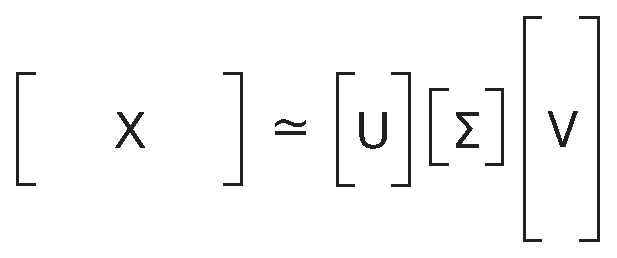
\includegraphics[width=0.5\textwidth]{images/svd.eps}
    \caption{Truncated SVD represented graphically; matrices size proportions are kept intact}
    \label{fig:svd}
\end{figure}

\begin{figure}[ht]
    \centering
    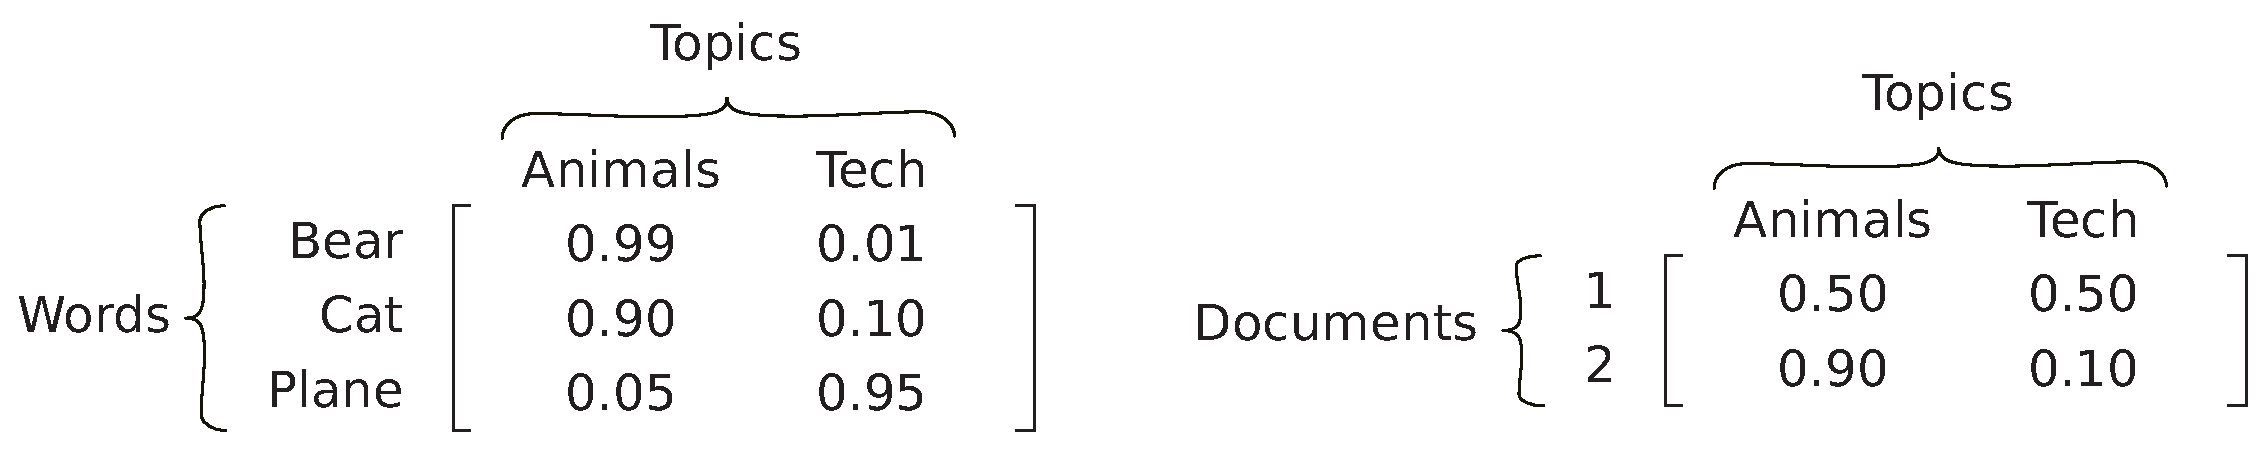
\includegraphics[width=\textwidth]{images/topic-mat.eps}
    \caption{Example of a term-topic and a document-topic matrix.}
    \label{fig:topicmat}
\end{figure}

\section{Latent Dirichlet Allocation (LDA)}
LDA makes the same assumptions about topics as LSA but unlike the latter, it views topics and documents in a probabilistic way.
In particular, a document is a categorical distribution over topics $\theta_d$ and a topic is a categorical distribution over words $\beta_i$.
The probability of sampling a document is instead modelled as a Dirichlet distribution $Dir(\alpha)$.

A major drawback of LDA is that the number of topics is assumed to be known a-priori and treated as a hyperparameter.

Variants of this model are present in the literature: in this chapter, we use \cite{10.1145/2107736.2107741} and \cite{DBLP:journals/jmlr/BleiNJ03} as a reference.

\subsection{Generative process} \label{gp}
In this section we describe LDA by its generative process, assuming we have already obtained the parameters of the model.

We define:
\begin{itemize}
    \item $\boldsymbol{\beta_{1:K}}$: $K$ topics, where each topic $\beta_i$ is a distribution over the terms in the vocabulary
    \item $\boldsymbol{\theta_d}$: a document $d$ described as a categorical distribution over topics, where $\theta_{d,k}$ is the topic proportion for topic $k$ in document $d$
    \item $\boldsymbol{w_{d}}$: observed words of document $d$, where $w_{d,n}$ is the word in position $n$ of document $d$
\end{itemize}

The generation of $M$ documents with $N$ words each can be summarized as:
\begin{enumerate}
    \item $\theta_d \sim Dir(\alpha)$: pick a document
    \item $z_{d,n} \sim \mathit{Mult}(\theta_d)$: sample a topic
    \item $w_{d,n} \sim \beta_{z_{d,n}}$: pick a term
    \item use that term as a word for the document you want to generate
    \item loop $N$ times to step 2
    \item loop $M$ times to step 1
\end{enumerate}

LDA is a probabilistic graphical model and it is represented graphically in Figure \ref{fig:lda}.

The joint distribution is:
\begin{equation*}
    \begin{split}
        p(\theta, z, w | \alpha, \beta) & = \prod_d p_d(\theta, z, w | \alpha, \beta) \\
        & = \prod_d [p(\theta_d | \alpha) \prod_n p(z_{d,n} | \theta_d) p(w_{d, n} | \beta, z_{d,n})]
    \end{split}
\end{equation*}

Given the distributions explained before, we can state that:
\[ p(\theta_d | \alpha) = \frac{1}{B(\alpha)} \prod_{k=1}^K \theta_{d,k}^{\alpha_k - 1} \]
\[ p(z_{d,n} | \theta_d) = \theta_{d, z_{d,n}} \]
\[ p(w_{d,n} | z_{d,n}, \beta) = \beta_{z_{d,n},w_{d,n}} \]

\begin{figure}[ht]
    \centering
    \subfigure{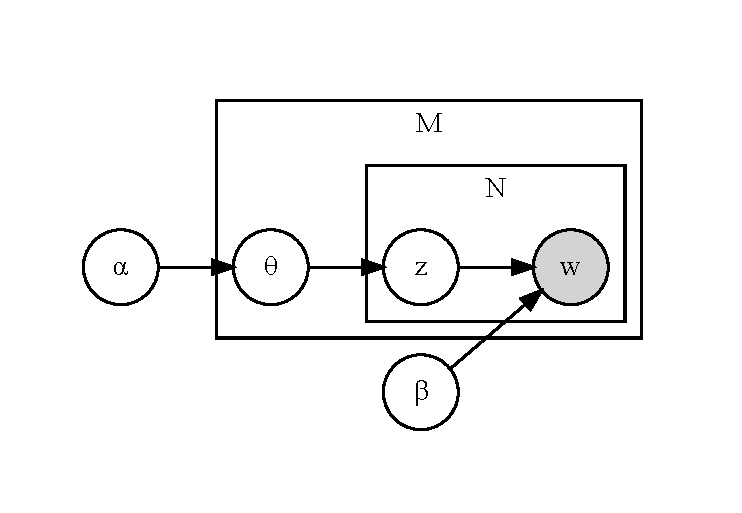
\includegraphics[height=150px]{images/lda.pdf}}
    \subfigure{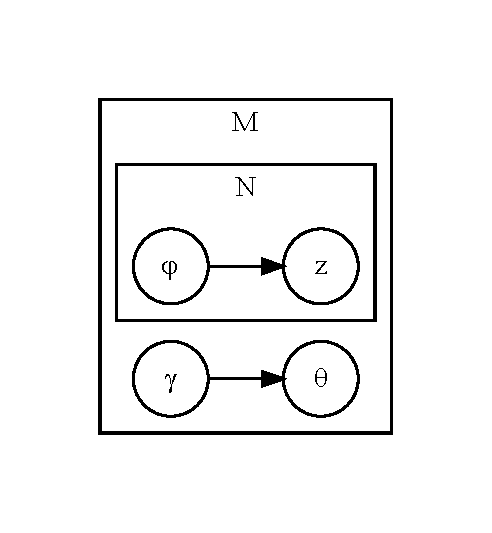
\includegraphics[height=150px]{images/lda-vi.pdf}}
    \caption{Graphical model representation of LDA (left) and graphical model representation of the variational distribution (right). Nodes are random variables, shaded if observed. An edge denotes a dependence between two random variables. Plates denote multiplicity.}
    \label{fig:lda}
\end{figure}

\subsection{Model inference} \label{modelinference}
The goal of LDA is to automatically discover topics over a collection of documents.
Since only words are observed, topics are considered latent variables.

Note that inference in this case can be seen as the reverse of the generative process explained in Section \ref{gp}.

Mathematically speaking, inference becomes a question of computing the posterior distribution:
\[ p(\theta, z | w, \alpha, \beta) = \frac{p(\theta, z, w | \alpha, \beta)}{p(w| \alpha, \beta)} \]

The denominator $p(w_{1:D} | \alpha, \beta)$ is the probability of observing the corpus under all possible topic model combinations
and thus intractable to compute.
For this reason, in this section we approximate the posterior distribution through a variational method
(see Appendix \ref{vi}).
In particular, we set $q$ as:
\begin{equation*}
    \begin{split}
        q(\theta, z | \gamma, \phi) & = \prod_d q_d(\theta, z | \gamma, \phi) \\
        & = \prod_d q_d(\theta | \gamma) q_d(z | \phi) \\
        & = \prod_d [q(\theta_d | \gamma_d) \prod_n q(z_{d,n} | \phi_{d,n})]
    \end{split}
\end{equation*}
$q(\theta_d | \gamma_d)$ is governed by a Dirichlet distribution, while $q(z_{d,n} | \phi_{d,n})$ by a Categorical distribution.
Its graphical representation can be seen in Figure \ref{fig:lda}.

To do model inference from a collection of documents, we start defining the ELBO function:
\begin{equation*}
    \begin{split}
        \ln[\prod_d p_d(w | \alpha, \beta)] & \geq
        \E_q \{ \ln[p(w, \theta, z | \alpha, \beta)] - \ln[q(\theta, z | \gamma, \phi)] \} \\
        & = \E_q \{ \ln[\prod_d p_d(w, \theta, z | \alpha, \beta)] - \ln[ \prod_d q_q(\theta, z | \gamma, \phi)] \} \\
        & = \E_q \{ \sum_d \ln[p_d(w, \theta, z | \alpha, \beta)] - \sum_d \ln[q_q(\theta, z | \gamma, \phi)] \} \\
        & = \sum_d \E_q \{ \ln[p_d(w, \theta, z | \alpha, \beta)] - \ln[q_q(\theta, z | \gamma, \phi)] \} \\
        & = \sum_d \E_{q_d} \{ \ln[p_d(w, \theta, z | \alpha, \beta)] - \ln[q_d(\theta, z | \gamma, \phi)] \} \\
    \end{split}
\end{equation*}

First, we fix $\alpha$ and $\beta$ to find the best $q(\theta, z | \gamma, \phi)$ that minimizes the KL-divergence between $q$ and $p$.
Then, we fix $(\theta, z | \gamma, \phi)$ to find the best $\alpha$ and $\beta$ that maximize the lower bound.
This process, if done iteratively, converges to a local optimum.
In the literature, it is called expectation-maximization (EM).

Since constrained maximization and
the Newton-Raphson algorithm are needed to solve the problem
instead of traditional variational inference,
we intentionally present only a hasty description of the update algorithm:
\begin{enumerate}
    \item initialize $\beta$ randomly, set each $\phi_{d,n}$ as $\frac{1}{K}$ and each $\gamma_d$ as $\alpha_d + \frac{N}{K}$
    \item for each document, update the local latent variables $\gamma$ and $\phi$ until convergence
    \item update the global variables $\beta$ and $\alpha$ for the entire corpus until convergence
    \item loop to 2 until convergence
\end{enumerate}

The updates are affected by:
\begin{itemize}
    \item $\phi_{d,n,k} \propto \beta_{k, w_n} e^{\Psi(\gamma_{d,k}) - \sum_j^K \Psi(\gamma_{d,j})}$, where $\Psi$ is the first derivative of the logarithm of the gamma function
    \item $\gamma_{d,k} = \alpha_k + \sum_n \phi_{d,n,k}$
    \item $\beta_{k,j} \propto \sum_d \sum_n \mathbb{1}_{[w_{d,n} == j]} \phi_{d,n,k}$
    \item $\frac{\partial \mathit{ELBO}}{ \partial \alpha_k} = \sum_d [ \Psi(\sum_j^K \alpha_j) - \Psi(\alpha_k) + \Psi(\gamma_{d,k}) - \Psi(\sum_j^K \gamma_{d,j})]$
\end{itemize}

The interested reader can find more details looking at Appendix A of \cite{DBLP:journals/jmlr/BleiNJ03}.

Note that step 2 can be parallelized: each document has its local variables that are conditionally independent
of the other local variables and data in different documents.

After the execution of the algorithm, each row $d$ of the final document-topic matrix can be obtained using the Maximum Likelihood Estimation method over $q(\theta_d | \gamma_d)$.

\subsection{Sparsity considerations} \label{sparsity_lda}
Using the Dirichlet governed by the $\alpha$ parameter to induce sparsity
allows us to have documents described by fewer topics than using an uninformative prior.
The same reasoning can be applied to topics, introducing a Dirichlet that governs the
probability of having a topic with a particular set of terms.

Inducing sparsity combined with the number of topics much less than the number of documents
lower the risk of obtaining two different topics with a similar distribution of words.


\section{Online LDA}
A major drawback of LDA is the impossibility to scale as the data grows:
each iteration of the algorithm requires an entire scan of the corpus, which is computationally expensive.

For this reason, \cite{NIPS2010_3902} proposes an online learning variation based on the original LDA model.
This algorithm called online LDA does not need to store all documents together,
but they can arrive in a stream and be discarded after one look.

The main difference between the graphical model presented in Section \ref{modelinference} and this one
is that the latter assumes each $\beta_k$ sampled from a Dirichlet distribution as presented in Section \ref{sparsity_lda}:
\begin{equation}
    \beta_k \sim Dir(\eta)
\end{equation}
For this reason, $q$ becomes:
\begin{equation*}
    \begin{split}
        q(\beta, \theta, z| \lambda, \gamma, \phi) & = [\prod_k q_k(\beta | \lambda)] [\prod_d q_d(\theta, z | \gamma, \phi)] \\
        & = [\prod_k q(\beta_k | \lambda_k)] [\prod_d q_d(\theta | \gamma) q_d(z | \phi)] \\
        & = [\prod_k q(\beta_k | \lambda_k)] \{\prod_d [q(\theta_d | \gamma_d) \prod_n q(z_{d,n} | \phi_{d,n})]\}
    \end{split}
\end{equation*}
$q(\beta_k | \lambda_k)$ and $q(\theta_d | \gamma_d)$ are governed by a Dirichlet distribution, while $q(z_{d,n} | \phi_{d,n})$ by a Categorical distribution.

Due to that change compared to LDA, the ELBO is now:
\begin{equation*}
    \ln [p(w | \alpha, \eta)] \geq \E_q\{ \ln [p(w, z, \theta, \beta | \alpha, \eta)] - \ln[q(z, \theta, \beta | \gamma, \phi, \lambda)] \}
\end{equation*}
If we have $M$ documents, the ELBO can be factorized as:
\begin{equation*}
    \begin{split}
        \{\sum_{d=1}^M \E_{q} [ \ln p_d(w | \theta, z, \beta) + \ln p_d(z | \theta) & - \ln q_d(z | \phi) + \ln p_d(\theta | \alpha) - \ln q_d(\theta | \gamma)]\} \\
        & + \E_q[\ln p(\beta | \eta) - \ln q(\beta | \lambda)] = \\
        \{\sum_{d=1}^M \E_{q} [ \ln p_d(w | \theta, z, \beta) + \ln p_d(z | \theta) & - \ln q_d(z | \phi) + \ln p_d(\theta | \alpha) - \ln q_d(\theta | \gamma)] \\
        & + [\ln p(\beta | \eta) - \ln q(\beta | \lambda)]/M \} \\
    \end{split}
\end{equation*}

Similar to what we do for LDA, we could maximize the lower bound using coordinate ascent over the variational parameters.
As for LDA, it requires a full pass through the entire corpus at each iteration.

To fix this issue, we load documents in batches. For each batch $t$ of size $S$, we compute the local parameters $\phi_t$ and $\gamma_t$, holding $\lambda$ fixed.
Then, we compute an estimate of $\lambda$ related to that batch that we call $\tilde{\lambda}_t$
and we update $\lambda$ as a weighted average between its earlier value and $\tilde{\lambda}_t$:
\begin{equation*}
    \lambda = (1 - \rho_t) \lambda + \rho_t \tilde{\lambda}_t, \, \rho_t = (\tau_0 + t)^{-s}
\end{equation*}
where $\rho_t$ controls the importance of old values given the new ones. In particular:
\begin{itemize}
    \item increasing the value of $\tau_0 \geq 0$ slows down the initial updates
    \item $s \in (0.5, 1]$ controls the rate at which old information is forgotten
\end{itemize}

We can also incorporate updates of $\alpha$ and $\eta$:
\begin{itemize}
    \item $\alpha = \alpha - \rho_t \tilde{\alpha}_t$
    \item $\eta = \eta - \rho_t \tilde{\eta}_t$
\end{itemize}

The updates are affected by:
\begin{itemize}
    \item $\tilde{\alpha}_t = [\mathit{Hess}^{-1}(l)] [\nabla_{\alpha} l]$, where l is the sum of the ELBO of each document of the batch
    \item $\tilde{\eta}_t = [\mathit{Hess}^{-1}(l)] [\nabla_{\eta} l]$
    \item $\phi_{d,n,k} \propto e^{\E_q[\ln \theta_{d,k}] + \E_q[\ln \beta_{k, w_n}]}$
    \item $\gamma_{d,k} = \alpha_k + \sum_n \phi_{d,n,k}$
    \item $\tilde{\lambda}_{t,k,n} = \eta_k + \frac{D}{|S|} \sum_{d = t \cdot S}^{(t+1) S - 1} \phi_{d,n,k} $
\end{itemize}

Note that if the batch size $|S|$ is equal to one, the algorithm becomes online.

After the execution of the algorithm, each row $d$ of the final document-topic matrix
can be obtained using the Maximum Likelihood Estimation method over $q(\theta_d | \gamma_d)$.
The same reasoning can be applied for topics, using MLE over $q(\beta_k | \lambda_k)$.


\section{Hierarchical Dirichlet process (HDP)}

HDP was proposed in \cite{DBLP:journals/jmlr/WangPB11}
as a way to overcome the problem of choosing the number
of topics in LDA and derived methods
while using an online variational inference algorithm.
In particular, the number of topics is inferred from data.

Since this method uses the Dirichlet process, we need to introduce it first.

\subsection{Dirichlet process (DP)} \label{dipro}
The Dirichlet process can be used as a generalization of the Dirichlet distribution
which does not have a fixed number of topics.

Formally, it is defined as a two parameter distribution $\mathit{DP}(\alpha, H)$,
where $\alpha$ is the concentration parameter and H is the base distribution.

To get an intuition on how it works, it can be viewed as a black-box
which takes as input a continuous distribution $H$ and produces a discrete distribution $G_0$
whose similarity with $H$ is governed by $\alpha$: as $\alpha \to \infty$, $G_0 = H$.

The procedure of generating $G_0$ can be described through the stick-breaking process.
The basic idea is that you have a stick of unit length and you break it off.
At each iteration $i$, you pick the remaining part of the stick and you break it off again and again.
The entire process takes an infinite number of steps since you can always break off the remaining part
of a stick, ending up to smaller and smaller pieces.

More formally:
\begin{equation*}
    \beta_k' \sim \mathit{Beta}(1, \alpha)
\end{equation*}
\begin{equation*}
    \beta_k = \beta_k' \prod_{l=1}^{k-1} (1 - \beta_l')
\end{equation*}
where $\beta_k'$ is the percentage of the remaining stick that is break off
and $\beta_k$ is the size of the broken part of the stick after step $k$.
All $\beta_k$ are then used as weights:

\begin{equation*}
    \phi_k \sim H
\end{equation*}
\begin{equation*}
    G(x) = \sum_{k=1}^{\infty} \mathbb{1}_{[x == \phi_k]} \beta_k
\end{equation*}

\subsection{HDP nesting DPs}
Using HDP instead of LDA or Online LDA requires the definition of a new model.
First, we will describe the generative process.
Then, we will analyse the steps of model inference.

\subsubsection{Generative process}
The model is composed of two layers:
\begin{itemize}
    \item $\boldsymbol{G_d | G_0 \sim \mathit{DP}(\alpha, G_0)}$: each document $d$ is described by its own DP $G_d$
    \item $\boldsymbol{G_0 \sim \mathit{DP}(\gamma, H)}$: each $G_d$ is sampled from another DP $G_0$; in this way all $G_d$ have the same atoms and they differ only in their weights
\end{itemize}
where $H$ is a symmetric Dirichlet distribution over the vocabulary.

The stick-breaking construction of $G_0$ is the same as the one presented in Section \ref{dipro}.
The one for each $G_d$ is instead:
\begin{itemize}
    \item $c_{d,k} \sim \mathit{Mult}(\beta)$
    \item $\pi_{d,k}' \sim \mathit{Beta(1, \alpha)}$
    \item $\pi_{d,k} = \pi_{d,k}' \prod_{l=1}^{k-1} (1 - \pi_{d,l}')$
    \item $G_j(x) = \sum_{k=1}^{\infty} \mathbb{1}_{[x == \phi_{c_{d,k}}]} \pi_{d,k}$
\end{itemize}

The generation of a word in position $n$ is then:
\begin{itemize}
    \item $z_{d,n} \sim \mathit{Mult}(\pi_d)$
    \item $\theta_{d,n} = \phi_{c_{d,z_{d,n}}}$
    \item $w_{d,n} \sim \mathit{Mult}(\theta_{d,n})$
\end{itemize}

The plate notation of HDP is represented in Figure \ref{fig:hdp}.

\begin{figure}[h]
    \centering
    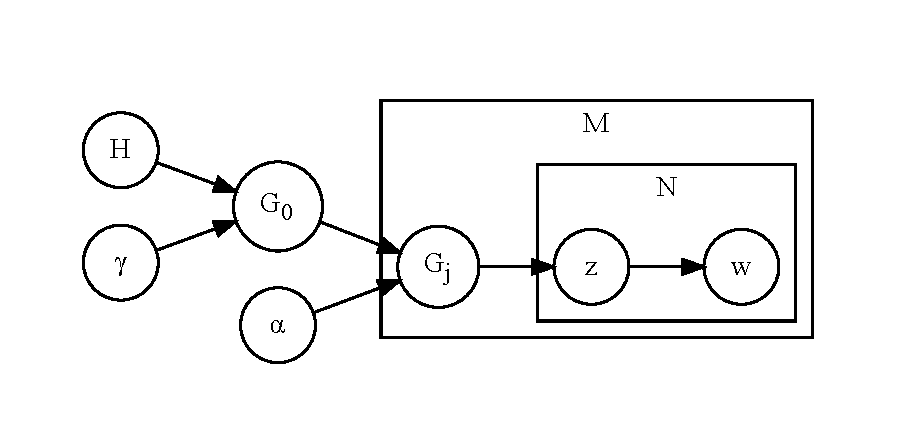
\includegraphics[width=0.6\textwidth]{images/hdp.pdf}
    \caption{Graphical model representation of HDP.}
    \label{fig:hdp}
\end{figure}

\subsubsection{Model inference}
Due to the fact that this process requires an infinite number of steps,
truncation is needed to view the generative process and the inference as algorithms.
In particular, we set a maximum number of global topics $K$ and a maximum number of local topics $T$.
Note that a reasonable choice is to set $T \ll K$ since the number of topics needed for a single document is
less than the number of topics required for the full corpus.

Our variational distribution is:
\begin{equation*}
    q(\beta', \pi', c, z, \phi) = q(\beta' | u, v) q(\pi' | a, b) q(c | \varphi) q(z | \zeta) q(\phi | \lambda)
\end{equation*}
Factorizing it results in:
\begin{itemize}
    \item $q(c | \varphi) = \prod_d \prod_{t=1}^T q(c_{d,t} | \varphi_{d,t})$
    \item $q(z | \zeta) = \prod_d \prod_n q(z_{d,n} | \zeta_{d,n})$
    \item $q(\phi | \lambda) = \prod_{k=1}^{K} q(\phi_k | \lambda_k)$
    \item $q(\beta' | u, v) = \prod_{k=1}^{K-1} q(\beta_k' | u_k, v_k)$
    \item $q(\pi' | a, b) = \prod_d \prod_{t=1}^{T-1} q(\pi_{d,t}' | a_{d,t}, b_{d,t})$
\end{itemize}
where $q(\beta_K' = 1) = 1$ and $\forall d \; q(\pi_{d,T}' = 1) = 1$.

As we did for LDA and Online LDA we take derivatives of the ELBO
with respect to each variational parameter.
The results are both document-level updates obtained using coordinate ascent
and corpus-level updates computed using gradient ascent.
These updates can be performed in an online fashion,
computing local updates only for a small part of documents
for each iteration and then performing the corpus-level updates using a noisy estimation
of the gradient.
Since the updates and the steps required to obtain them are similar to previous methods,
we deliberatively removed them from the description of HDP. However, the interested reader can
find all the details at \cite{DBLP:journals/jmlr/WangPB11}.